
\documentclass[letterpaper,hide notes,xcolor={table,svgnames},pdftex,10pt]{beamer}
\def\showexamples{t}


%\usepackage[svgnames]{xcolor}

%% Demo talk
%\documentclass[letterpaper,notes=show]{beamer}

\usecolortheme{crane}
\setbeamertemplate{navigation symbols}{}

\usetheme{MyPittsburgh}
%\usetheme{Frankfurt}

%\usepackage{tipa}

\usepackage{hyperref}
\usepackage{graphicx,xspace}
\usepackage[normalem]{ulem}
\usepackage{multicol}
\usepackage{amsmath,amssymb,amsthm,graphicx,xspace}
\newcommand\SF[1]{$\bigstar$\footnote{SF: #1}}

\usepackage[default]{sourcesanspro}
\usepackage[T1]{fontenc}
\usepackage[scaled]{beramono}
\usepackage{tikzpagenodes}

\newcounter{tmpnumSlide}
\newcounter{tmpnumNote}


% old question code
%\newcommand\question[1]{{$\bigstar$ \small \onlySlide{2}{#1}}}
% \newcommand\nquestion[1]{\ifdefined \presentationonly \textcircled{?} \fi \note{\par{\Large \textbf{?}} #1}}
% \newcommand\nanswer[1]{\note{\par{\Large \textbf{A}} #1}}


 \newcommand\mnote[1]{%
   \addtocounter{tmpnumSlide}{1}
   \ifdefined\showcues {~\tiny\fbox{\arabic{tmpnumSlide}}}\fi
   \note{\setlength{\parskip}{1ex}\addtocounter{tmpnumNote}{1}\textbf{\Large \arabic{tmpnumNote}:} {#1\par}}}

\newcommand\mmnote[1]{\note{\setlength{\parskip}{1ex}#1\par}}

%\newcommand\mnote[2][]{\ifdefined\handoutwithnotes {~\tiny\fbox{#1}}\fi
% \note{\setlength{\parskip}{1ex}\textbf{\Large #1:} #2\par}}

%\newcommand\mnote[2][]{{\tiny\fbox{#1}} \note{\setlength{\parskip}{1ex}\textbf{\Large #1:} #2\par}}

\newcommand\mquestion[2]{{~\color{red}\fbox{?}}\note{\setlength{\parskip}{1ex}\par{\Large \textbf{?}} #1} \note{\setlength{\parskip}{1ex}\par{\Large \textbf{A}} #2\par}\ifdefined \presentationonly \pause \fi}

\newcommand\blackboard[1]{%
\ifdefined   \showblackboard
  {#1}
  \else {\begin{center} \fbox{\colorbox{blue!30}{%
         \begin{minipage}{.95\linewidth}%
           \hspace{\stretch{1}} Some space intentionally left blank; done at the blackboard.%
         \end{minipage}}}\end{center}}%
         \fi%
}



%\newcommand\q{\tikz \node[thick,color=black,shape=circle]{?};}
%\newcommand\q{\ifdefined \presentationonly \textcircled{?} \fi}

\usepackage{listings}
\lstset{basicstyle=\footnotesize\ttfamily,
	breaklines=true,
	aboveskip=15pt,
  	belowskip=15pt,
	frame=lines,
	numbers=left, basicstyle=\scriptsize, numberstyle=\tiny, stepnumber=0, numbersep=2pt
}

\usepackage{siunitx}
\newcommand\sius[1]{\num[group-separator = {,}]{#1}\si{\micro\second}}
\newcommand\sims[1]{\num[group-separator = {,}]{#1}\si{\milli\second}}
\newcommand\sins[1]{\num[group-separator = {,}]{#1}\si{\nano\second}}
\sisetup{group-separator = {,}, group-digits = true}

%% -------------------- tikz --------------------
\usepackage{tikz}
\usetikzlibrary{positioning}
\usetikzlibrary{arrows,backgrounds,automata,decorations.shapes,decorations.pathmorphing,decorations.markings,decorations.text,decorations.pathreplacing}

\tikzstyle{place}=[circle,draw=blue!50,fill=blue!20,thick, inner sep=0pt,minimum size=6mm]
\tikzstyle{transition}=[rectangle,draw=black!50,fill=black!20,thick, inner sep=0pt,minimum size=4mm]

\tikzstyle{block}=[rectangle,draw=black, thick, inner sep=5pt]
\tikzstyle{bullet}=[circle,draw=black, fill=black, thin, inner sep=2pt]

\tikzstyle{pre}=[<-,shorten <=1pt,>=stealth',semithick]
\tikzstyle{post}=[->,shorten >=1pt,>=stealth',semithick]
\tikzstyle{bi}=[<->,shorten >=1pt,shorten <=1pt, >=stealth',semithick]

\tikzstyle{mut}=[-,>=stealth',semithick]

\tikzstyle{treereset}=[dashed,->, shorten >=1pt,>=stealth',thin]

\usepackage{ifmtarg}
\usepackage{xifthen}
\makeatletter
% new counter to now which frame it is within the sequence
\newcounter{multiframecounter}
% initialize buffer for previously used frame title
\gdef\lastframetitle{\textit{undefined}}
% new environment for a multi-frame
\newenvironment{multiframe}[1][]{%
\ifthenelse{\isempty{#1}}{%
% if no frame title was set via optional parameter,
% only increase sequence counter by 1
\addtocounter{multiframecounter}{1}%
}{%
% new frame title has been provided, thus
% reset sequence counter to 1 and buffer frame title for later use
\setcounter{multiframecounter}{1}%
\gdef\lastframetitle{#1}%
}%
% start conventional frame environment and
% automatically set frame title followed by sequence counter
\begin{frame}%
\frametitle{\lastframetitle~{\normalfont(\arabic{multiframecounter})}}%
}{%
\end{frame}%
}
\makeatother

\makeatletter
\newdimen\tu@tmpa%
\newdimen\ydiffl%
\newdimen\xdiffl%
\newcommand\ydiff[2]{%
    \coordinate (tmpnamea) at (#1);%
    \coordinate (tmpnameb) at (#2);%
    \pgfextracty{\tu@tmpa}{\pgfpointanchor{tmpnamea}{center}}%
    \pgfextracty{\ydiffl}{\pgfpointanchor{tmpnameb}{center}}%
    \advance\ydiffl by -\tu@tmpa%
}
\newcommand\xdiff[2]{%
    \coordinate (tmpnamea) at (#1);%
    \coordinate (tmpnameb) at (#2);%
    \pgfextractx{\tu@tmpa}{\pgfpointanchor{tmpnamea}{center}}%
    \pgfextractx{\xdiffl}{\pgfpointanchor{tmpnameb}{center}}%
    \advance\xdiffl by -\tu@tmpa%
}
\makeatother
\newcommand{\copyrightbox}[3][r]{%
\begin{tikzpicture}%
\node[inner sep=0pt,minimum size=2em](ciimage){#2};
\usefont{OT1}{phv}{n}{n}\fontsize{4}{4}\selectfont
\ydiff{ciimage.south}{ciimage.north}
\xdiff{ciimage.west}{ciimage.east}
\ifthenelse{\equal{#1}{r}}{%
\node[inner sep=0pt,right=1ex of ciimage.south east,anchor=north west,rotate=90]%
{\raggedleft\color{black!50}\parbox{\the\ydiffl}{\raggedright{}#3}};%
}{%
\ifthenelse{\equal{#1}{l}}{%
\node[inner sep=0pt,right=1ex of ciimage.south west,anchor=south west,rotate=90]%
{\raggedleft\color{black!50}\parbox{\the\ydiffl}{\raggedright{}#3}};%
}{%
\node[inner sep=0pt,below=1ex of ciimage.south west,anchor=north west]%
{\raggedleft\color{black!50}\parbox{\the\xdiffl}{\raggedright{}#3}};%
}
}
\end{tikzpicture}
}


%% --------------------

%\usepackage[excludeor]{everyhook}
%\PushPreHook{par}{\setbox0=\lastbox\llap{MUH}}\box0}

%\vspace*{\stretch{1}

%\setbox0=\lastbox \llap{\textbullet\enskip}\box0}

\setlength{\parskip}{\fill}

\newcommand\noskips{\setlength{\parskip}{1ex}}
\newcommand\doskips{\setlength{\parskip}{\fill}}

\newcommand\xx{\par\vspace*{\stretch{1}}\par}
\newcommand\xxs{\par\vspace*{2ex}\par}
\newcommand\tuple[1]{\langle #1 \rangle}
\newcommand\code[1]{{\sf \footnotesize #1}}
\newcommand\ex[1]{\uline{Example:} \ifdefined \presentationonly \pause \fi
  \ifdefined\showexamples#1\xspace\else{\uline{\hspace*{2cm}}}\fi}

\newcommand\ceil[1]{\lceil #1 \rceil}


\AtBeginSection[]
{
   \begin{frame}
       \frametitle{Outline}
       \tableofcontents[currentsection]
   \end{frame}
}



\pgfdeclarelayer{edgelayer}
\pgfdeclarelayer{nodelayer}
\pgfsetlayers{edgelayer,nodelayer,main}

\tikzstyle{none}=[inner sep=0pt]
\tikzstyle{rn}=[circle,fill=Red,draw=Black,line width=0.8 pt]
\tikzstyle{gn}=[circle,fill=Lime,draw=Black,line width=0.8 pt]
\tikzstyle{yn}=[circle,fill=Yellow,draw=Black,line width=0.8 pt]
\tikzstyle{empty}=[circle,fill=White,draw=Black]
\tikzstyle{bw} = [rectangle, draw, fill=blue!20, 
    text width=4em, text centered, rounded corners, minimum height=2em]
    
    \newcommand{\CcNote}[1]{% longname
	This work is licensed under the \textit{Creative Commons #1 3.0 License}.%
}
\newcommand{\CcImageBy}[1]{%
	\includegraphics[scale=#1]{creative_commons/cc_by_30.pdf}%
}
\newcommand{\CcImageSa}[1]{%
	\includegraphics[scale=#1]{creative_commons/cc_sa_30.pdf}%
}
\newcommand{\CcImageNc}[1]{%
	\includegraphics[scale=#1]{creative_commons/cc_nc_30.pdf}%
}
\newcommand{\CcGroupBySa}[2]{% zoom, gap
	\CcImageBy{#1}\hspace*{#2}\CcImageNc{#1}\hspace*{#2}\CcImageSa{#1}%
}
\newcommand{\CcLongnameByNcSa}{Attribution-NonCommercial-ShareAlike}

\newenvironment{changemargin}[1]{% 
  \begin{list}{}{% 
    \setlength{\topsep}{0pt}% 
    \setlength{\leftmargin}{#1}% 
    \setlength{\rightmargin}{1em}
    \setlength{\listparindent}{\parindent}% 
    \setlength{\itemindent}{\parindent}% 
    \setlength{\parsep}{\parskip}% 
  }% 
  \item[]}{\end{list}} 




\title{Lecture 33 --- Applying Queueing Theory}

\author{Jeff Zarnett\\ \small \texttt{jzarnett@uwaterloo.ca}}
\institute{Department of Electrical and Computer Engineering \\
  University of Waterloo}
\date{\today}


\begin{document}

\begin{frame}
  \titlepage

 \end{frame}




\begin{frame}
\frametitle{Little's Law}

Little's Law says the average number of jobs in the system equals the product the average arrival rate into the system and the average arrival time in the system. 

Let's start with an open system. The law, written more formally:

\begin{center}
	$E[N] = \lambda E[T]$
\end{center}

\end{frame}



\begin{frame}
\frametitle{Little's Law}

\begin{center}
	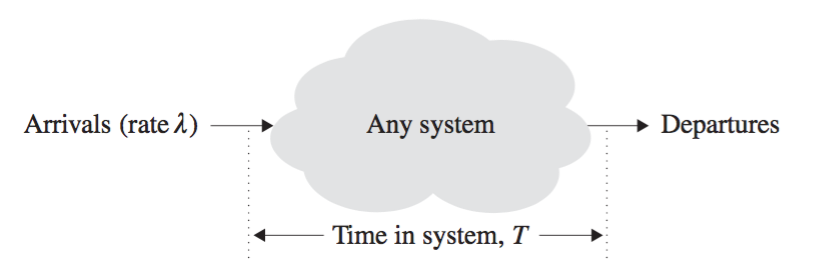
\includegraphics[width=0.8\textwidth]{images/littleslaw.png}
\end{center}

\end{frame}



\begin{frame}
\frametitle{Observations on Little's Law}

Note that we don't need to know anything about the arrival process the service time distribution, network topology, etc. 

It seems intuitive that this is the case (or it should). 

\end{frame}



\begin{frame}
\frametitle{Restaurant Analogy}

Imagine a fast food restaurant: they make money by quick turnaround time. 

They get people out of the place quickly (low $E[T]$) and accordingly they don't require a lot of seating (low $E[N]$). 

A sit down restaurant is the opposite though; people leave slowly (high $E[T]$) and therefore the restaurant needs lots of seating (more $E[N]$). 


\end{frame}



\begin{frame}
\frametitle{FCFS Version}

If you prefer to think of this in a single FCFS queue version, imagine a customer arrives and sees $E[N]$ jobs ahead of her in the queue. 

The expected time for each customer to complete is $1/\lambda$, because the average rate of completions is $\lambda $. 

So we can approximate $E[T]$ as being roughly $\dfrac{1}{\lambda}E[N]$.

\end{frame}



\begin{frame}
\frametitle{Little's Law for Closed Systems}

Remember that for closed systems, we have a rule that says there is $N$ jobs in process at any given time (the multiprocessing level of the system). 

If the system is ergodic, then $N = X \cdot E[T]$.

 This assumes that there is zero think time.

\end{frame}



\begin{frame}
\frametitle{Users Ruin Everything}

If we do have to deal with the vagaries of users and this time, then we care more about the response time $E[R]$. 

So for a terminal-driven system, the expected response time is $E[R] = \dfrac{N}{X} - E[Z]$. 

\end{frame}



\begin{frame}
\frametitle{M/M/1}

Probabilistic processes are described according to their models, which will probably one of the three:

\begin{enumerate}
	\item Deterministic (D)	
	\item Markov (M)
	\item General (G)
\end{enumerate}

\end{frame}



\begin{frame}
\frametitle{Markov Processes}

We're going to focus on Markov processes. 

It means that the number of arrivals follow the Poisson distribution.

The inter-arrival times follow the exponential distribution. 

Service times follow the exponential distribution too. 

\end{frame}



\begin{frame}
\frametitle{Kendall Notation}

Those letters we saw are part of Kendall notation. 

It has six symbols, written in a specific order, separated by slashes. 

The order is $\alpha / \sigma / m / \beta / N / Q$. 

\end{frame}



\begin{frame}
\frametitle{Kendall Notation}

\begin{center}
\begin{tabular}{l|l} 
	\textbf{Symbol} & \textbf{Meaning} \\ \hline
	$\alpha$ & The type of distribution (Markov, General, Deterministic) \\ \hline
	$\sigma$ & The type of probability distribution for service time \\ \hline
	$m$ & Number of servers \\ \hline
	$\beta$ & Buffer size \\ \hline
	$N$ & Allowed population size (finite or infinite) \\ \hline
	$Q$ & Queueing policy \\ 
\end{tabular}
\end{center}

\end{frame}



\begin{frame}
\frametitle{Why is abbreviation such a long word?}

We often leave off the last three, assuming that there is an infinite buffer, infinite population, and a FIFO queueing policy. 

If that is the case, then we have only three values. 

Those three then produce the ``M/M/1'' and ``M/M/k'' symbols. 

``M/M/1'' means a Markov arrival process, exponential queueing system, and a single server. 

When there are $k$ servers, then, of course the 1 is replaced with the $k$. 

\end{frame}



\begin{frame}
\frametitle{Utilization}

We should also think about utilization, denoted $\rho$. 

It is a fraction between 0 and 1 and it is simply the amount of time that the server is busy. 

We talked about this earlier in an informal way, but now we can actually calculate it! 

$\rho = \lambda \times s$.

\end{frame}



\begin{frame}
\frametitle{M/M/1 Formulae}

For M/M/1 systems: 

The completion time average $T_{q}$ is $\dfrac{s}{(1-\rho)}$

The average length of the queue $W$ is $\dfrac{\rho^{2}}{1-\rho}$.

\end{frame}



\begin{frame}
\frametitle{Queuing Theory Example}

We have a server that completes a request, on average, in 10~ms. 

The time to complete a request is exponentially distributed. 

Over a period of 30 minutes, 117~000 jobs arrive. 

So this is a M/M/1 situation. 

How long did it take to complete the average request? 

What is the average length of the queue?

\end{frame}



\begin{frame}
\frametitle{Queueing Theory Example}

The service time $s$ is given as $0.01s$, the arrival rate is 65 requests per second. 

So we can calculate $\rho = 0.01 \times 65 = 0.65$. 

So we have what we need to plug and chug using the formulae from above. 

The time to complete the average request is 28.6~ms. 

The average length of the queue is 1.21.

\end{frame}



\begin{frame}
\frametitle{Queueing Theory Example}

What about the number of jobs in the system? 

The value $Q$ gives the average number of jobs, including the waiting jobs and the ones being served.  

The probability that there are exactly $x$ jobs in the system at any time is given by the formula: $(1-\rho)\rho^{x}$.

\end{frame}



\begin{frame}
\frametitle{Queueing Theory Example}

The probability that the number of jobs is less than or equal to $n$ is then given by: 

$\sum\limits_{i=0}^{n}(1-\rho)\rho^{i}$.

For more than $n$ at a time, from $n-1$ to infinity... Or...

$1 - \sum\limits_{i=0}^{n}(1-\rho)\rho^{i}$.

\end{frame}



\begin{frame}
\frametitle{M/M/k}

Now let us take it to multiple servers. 

We will say jobs arrive at a single queue and then when a server is ready it will take the first job from the front of the queue. 

The servers are identical and jobs can be served by any server. 

So far, so simple. Sadly, the math just got harder. 

\end{frame}




\begin{frame}
\frametitle{M/M/k}

The server utilization for the server farm is now $\rho = \lambda s / N$.

To make our calculations a little easier, we want an intermediate value $K$:
\begin{center}
	$K = \cfrac{\sum_{i=0}^{N-1}\dfrac{(\lambda s)^{i}}{i!}}{{\sum_{i=0}^{N}\dfrac{(\lambda s)^{i}}{i!}}}$
\end{center}

$K$ is always less than 1. It has no intrinsic meaning.

\end{frame}

\begin{frame}
\frametitle{M/M/k}

What is the probability that all servers are busy? 

We represent this as $C$, the probability a new job will have to wait in the queue.

\begin{center}
	$C = \cfrac{1 - K}{1 - \dfrac{\lambda s K}{N}}$
\end{center}

The M/M/k formulae: 

\begin{center}
  $T_{q} = \dfrac{C s}{k(1 - \rho)} + s$ \qquad\qquad\qquad\qquad $W = C \dfrac{\rho}{1 - \rho}$
\end{center}


\end{frame}


\begin{frame}
\frametitle{Printer Example}

Suppose we have a printer that can complete an average print job in 2 min. 

Every 2.5 minutes, a user submits a job to the printer. 

How long does it take to get the print job on average? 

We're starting with a single printer, so the system is M/M/1. 

Service time $s$ is 2 minutes; the arrival rate $\lambda$ is $1/2.5 = 0.4$. 

So $\rho = \lambda \times s = 0.4 \times 2 = 0.8$. 

So $T_{q} = s / (1 - \rho ) = 2 / (1 -0.8 ) = 10$. 

Ten minutes to get the print job. Ouch.

\end{frame}



\begin{frame}
\frametitle{Executive Decision}

Here we have an opportunity to use the predictive power of queueing theory. 

Management is convinced that ten minute waits for print jobs is unreasonable, so we have been asked to decide what to do. 

Should we buy a second printer of the same speed, or should we sell the old one and buy a printer that is double the speed?

\end{frame}



\begin{frame}
\frametitle{New Printer}

The faster printer calculation is easy enough. 

Now $s = 1.0$ and $\lambda$ remains $0.4$, making $\rho = 0.4$. 

So rerunning the calculation: $T_{q} = s / (1 - \rho ) = 1 / (1 - 0.4 ) = 1.67$.

1:40 is a lot less time than 10:00! 

\end{frame}



\begin{frame}
\frametitle{Two Printer Solution}

The two printer solution is more complicated. So let us calculate $K$ as the intermediate value. 

\begin{center}
	$K = \cfrac{\sum_{i=0}^{N-1}\dfrac{(\lambda s)^{i}}{i!}}{{\sum_{i=0}^{N}\dfrac{(\lambda s)^{i}}{i!}}} = \cfrac{\dfrac{(\lambda s)^{0}}{0!} + \dfrac{(\lambda s)^{1}}{1!}}{\dfrac{(\lambda s)^{0}}{0!} + \dfrac{(\lambda s)^{1}}{1!} + \dfrac{(\lambda s)^{2}}{2!}} = 0.849057$
	
\end{center}

\end{frame}



\begin{frame}
\frametitle{Calculate!}

Now we can calculate $C$ as 0.22857 and $T_{q}$ as 2.57 minutes. 

Two observations jump out at us: 

(1) we doubled the number of printers, but now jobs are completed almost four times faster; and 

(2) the single fast printer is better, if utilization is low.

\end{frame}



\begin{frame}
\frametitle{Conditions}

That is an important condition: if utilization is low. 

At some point will the two printers be a better choice than the single fast one? 

What if both printers are used to the max (100\% load)...?

\end{frame}



\begin{frame}
\frametitle{Queueing for Performance}

The basic process is:

\begin{enumerate}
	\item Convert to common time units.
	\item Calculate the visitation ratios $V_{i}$.
	\item Calculate the device utilization $\rho_{i}$.
	\item Calculate the CPU service time.
	\item Calculate the device time.
	\item Find the bottleneck device.
	\item Calculate the maximum transaction rate.
	\item Calculate the average transaction time.
\end{enumerate}

\end{frame}



\begin{frame}
\frametitle{Queueing for Performance}

Let us execute this process on a web server system that serves 9~000 pages per hour. Here are the known values:

\begin{center}
\begin{tabular}{|l|l|l|l|l|l|l|} \hline
	\textbf{Device} & \textbf{Data/Hour} & \textbf{$\lambda$} & \textbf{$S$} & \textbf{$V$} & \textbf{$\rho$} & \textbf{$V \times S$} \\ \hline
	Webpages & 9~000 & & & & & \\ \hline
	CPU & & & & &  42\% & \\ \hline
	Disk 1 & 108~000 & & 11ms & & &\\ \hline
	Disk 2 & 72~000 & & 16ms & & &\\ \hline
	Network & 18~000 & & 23ms & & &\\ \hline
\end{tabular}
\end{center}

\end{frame}



\begin{frame}
\frametitle{Queueing for Performance}

Step one is to convert to common time units; in this case, seconds.

Let's also look at the $\lambda$ values - reported counts divided by seconds in the reporting period.

\begin{center}
\begin{tabular}{|l|l|l|l|l|l|l|} \hline
	\textbf{Device} & \textbf{Data/Hour} & \textbf{$\lambda$} & \textbf{$S$} & \textbf{$V$} & \textbf{$\rho$} & \textbf{$V \times S$} \\ \hline
	Webpages & 9~000 & 2.5 & & & & \\ \hline
	CPU & & & & & 42\% & \\ \hline
	Disk 1 & 108~000 & 30 & 0.011s  & & &\\ \hline
	Disk 2 & 72~000 & 20 & 0.016s & & &\\ \hline
	Network & 18~000 & 5 & 0.023s & & &\\ \hline
\end{tabular}
\end{center}

\end{frame}



\begin{frame}
\frametitle{Queuing for Performance}

The visitation ratio is the number of times a device is used in each transaction; divide use by number of transactions to get $V_{i}$ (you could also log this sort of thing). 

The visitation ratio of the CPU is the sum of all other visitation ratios.

\begin{center}
\begin{tabular}{|l|l|l|l|l|l|l|} \hline
	\textbf{Device} & \textbf{Data/Hour} & \textbf{$\lambda$} & \textbf{$S$} & \textbf{$V$} & \textbf{$\rho$} & \textbf{$V \times S$} \\ \hline
	Webpages & 9~000 & 2.5 & & 1 & & \\ \hline
	CPU & 207~000 & 57.5 &  & 23 & 42\% & \\ \hline
	Disk 1 & 108~000 & 30 & 0.011s  & 12& &\\ \hline
	Disk 2 & 72~000 & 20 & 0.016s & 8 & &\\ \hline
	Network & 18~000 & 5 & 0.023s & 2 & &\\ \hline
\end{tabular}
\end{center}

\end{frame}



\begin{frame}
\frametitle{Queueing for Performance}

Next, calculate device utilization: $\rho = \lambda \times s$. That is, arrival rate times service time.

\begin{center}
\begin{tabular}{|l|l|l|l|l|l|l|} \hline
	\textbf{Device} & \textbf{Data/Hour} & \textbf{$\lambda$} & \textbf{$S$} & \textbf{$V$} & \textbf{$\rho$} & \textbf{$V \times S$} \\ \hline
	Webpages & 9~000 & 2.5 & & 1 & & \\ \hline
	CPU & 207~000 & 57.5 &  & 23 & 42\% & \\ \hline
	Disk 1 & 108~000 & 30 & 0.011s  & 12& 0.33 &\\ \hline
	Disk 2 & 72~000 & 20 & 0.016s & 8 & 0.32 &\\ \hline
	Network & 18~000 & 5 & 0.023s & 2 & 0.115 &\\ \hline
\end{tabular}
\end{center}

\end{frame}



\begin{frame}
\frametitle{Queueing for Performance}

We can also get the service time of the CPU by rearrangement of the utilization formula to $s = \rho / \lambda$.

\begin{center}
\begin{tabular}{|l|l|l|l|l|l|l|} \hline
	\textbf{Device} & \textbf{Data/Hour} & \textbf{$\lambda$} & \textbf{$S$} & \textbf{$V$} & \textbf{$\rho$} & \textbf{$V \times S$} \\ \hline
	Webpages & 9~000 & 2.5 & & 1 & & \\ \hline
	CPU & 207~000 & 57.5 & 0.0073s & 23 & 0.42 & \\ \hline
	Disk 1 & 108~000 & 30 & 0.011s  & 12& 0.33 &\\ \hline
	Disk 2 & 72~000 & 20 & 0.016s & 8 & 0.32 &\\ \hline
	Network & 18~000 & 5 & 0.023s & 2 & 0.115 &\\ \hline
\end{tabular}
\end{center}

\end{frame}



\begin{frame}
\frametitle{Queuing for Performance}

And the device time is the final thing we can fill in for this table: $V_{i} \times S_{i}$ (just like the column header says!).

\begin{center}
\begin{tabular}{|l|l|l|l|l|l|l|} \hline
	\textbf{Device} & \textbf{Data/Hour} & \textbf{$\lambda$} & \textbf{$S$} & \textbf{$V$} & \textbf{$\rho$} & \textbf{$V \times S$} \\ \hline
	Webpages & 9~000 & 2.5 & & 1 & & \\ \hline
	CPU & 207~000 & 57.5 & 0.0073s & 23 & 0.42 & 0.168\\ \hline
	Disk 1 & 108~000 & 30 & 0.011s  & 12& 0.33 & 0.132\\ \hline
	Disk 2 & 72~000 & 20 & 0.016s & 8 & 0.32 & 0.128\\ \hline
	Network & 18~000 & 5 & 0.023s & 2 & 0.115 & 0.046\\ \hline
\end{tabular}
\end{center}

\end{frame}



\begin{frame}
\frametitle{Is It Useful?}

Did we need to complete the whole table? Probably not. 

In a practical sense what we cared about the most was the $\rho$ column -- utilization. 

The bottleneck device, i.e., the one that limits our maximum throughput, is the one that is the busiest. 

Thus, the one with the largest utilization. 

This application appears to be CPU bound; it has the highest utilization at 42\%, well ahead of disk 1 and disk 2. 

\end{frame}



\begin{frame}
\frametitle{Predicting the Maxes}

Having identified the bottleneck device as the CPU, we can make a prediction about the maximum rate of transactions (web page requests) we can serve. 

$\dfrac{1}{S_{i}V_{i}}$ or in this example, 5.95. 

This is also called saturation.

 If $\lambda$ exceeds this saturation point, we will not be able to keep up with incoming requests.

With this table we can also calculate the average transaction time: it is the sum of the $S_{i}V_{i}$ columns. 

In this example, it is 0.474 seconds. 


\end{frame}



\begin{frame}
\frametitle{It Gets Worse!}

The typical assumption is that we know the service times for each device. 

Unfortunately this is not true; usually performance monitoring gives us the average size of a device queue. 

So we had better apply queuing theory here.


\end{frame}



\begin{frame}
\frametitle{Queue Length}


The average size of a device's queue is $W$, and for a queue with characteristics M/M/1 then $W = \dfrac{\rho^{2}}{1-\rho}$. 

Combining the known $W$ with the average arrival rate $\lambda$, we can work out the service time. 

\begin{center}
$W = \dfrac{(\lambda s)^{2}}{1 - \lambda s}$


	$s = \cfrac{-w \pm \sqrt{w^{2}+4w}}{2\lambda}$
\end{center}



\end{frame}

\end{document}

